\graphicspath{{e05_Kondensator/}}

\clearpage
\begin{minipage}{0.8\textwidth}
  \chapter{Der Kondensator (E05)}
\end{minipage}
\begin{minipage}{0.2\textwidth}
  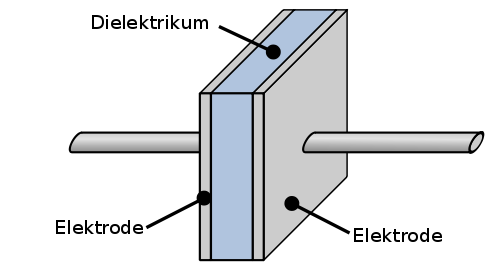
\includegraphics[width=0.9\textwidth]{Kondensator.png}
  \footnotemark
\end{minipage}
\footnotetext{Quelle unbekannt} % FIXME

%%%%%%%%%%%%%%%%%%%%%%%%%%%%%%%%%%%%%%%%%%%%%%%%%%%%%%%%%%%%%%%%%%%%%%%%
%% Theorie

\section{Theorie- und Prüfungsfragen}

\mucho{1}{TC206}
{
Drei Kondensatoren mit den Kapazitäten $C_1 = 0,1\mu F$, $C_2 = 150nF$ und $C_3 = 50000pF$ werden parallel geschaltet. Wie groß ist die Gesamtkapazität?
}%Frage
{$0,027\mu F$}%A
{$0,255\mu F$}%B
{$0,3\mu F$}%C
{$2,73nF$}%D
{C; $C_g = 100nF + 150nF + 50nF = 300nF = 0,3\mu F$}%Lösung


\mucho{2}{TD105}
{
Berechnen Sie die Gesamtkapazität der gemischten Schaltung.\\
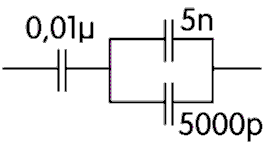
\includegraphics[scale=0.35]{TD105.png}
}%Frage
{$0,015nF$}%A
{$5nF$}%B
{$7,5nF$}%C
{$10nF$}%D
{B; $C_g = \dfrac{C_1 \cdot C_{2+3}}{C_1 + C_{2+3}} = \dfrac{10nF \cdot (5nF + 5nF)}{10nF + (5nF + 5nF)} = 5$}%Lösung

\mucho{3}{TD106}
{
Berechnen Sie die Gesamtkapazität der gemischten Schaltung. Gegeben: $C1 = 0,02\mu F$; $C2 = 10nF$; $C3 = 10000pF $ \\
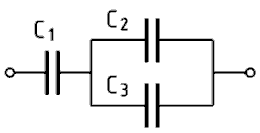
\includegraphics[scale=0.35]{TD106.png}
}%Frage
{$2,5nF$}%A
{$5nF$}%B
{$10nF$}%C
{$40nF$}%D
{C; $C_g = \dfrac{C_1 \cdot C_{2+3}}{C_1 + C_{2+3}} = \dfrac{20nF \cdot (10nF + 10nF)}{20nF + (10nF + 10nF)} = 10nF$}%Lösung

\mucho{4}{TD107}
{
Berechnen Sie die Gesamtkapazität der gemischten Schaltung. Gegeben: $C1 = 0,01 \mu F$; $C2 = 10 nF$; $C3 = 5000 pF$\\
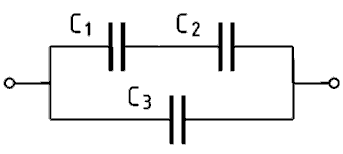
\includegraphics[scale=0.3]{TD107.png}
}%Frage
{$2,5 nF$}%A
{$5 nF$}%B
{$10 nF$}%C
{$0,015 nF$}%D
{C; $C_g = \dfrac{C_1 \cdot C_2}{C_1 + C_2} + C_3 = \dfrac{10nF \cdot 10nF}{10nF + 10nF} + 5nF = 10nF$}%Lösung

\mucho{5}{TC208}
{Mit zunehmender Frequenz}%Frage
{steigt der Wechselstromwiderstand des Kondensators.}%A
{sinkt der Wechselstromwiderstand des Kondensators.}%B
{steigt der Wechselstromwiderstand des Kondensators bis zu einem Maximum und sinkt dann wieder.}%C
{sinkt der Wechselstromwiderstand des Kondensators bis zu einem Minimum und steigt dann wieder.}%D
{B; $X_C = \dfrac{1}{2\pi \cdot f \cdot C}$}%Lösung


\mucho{6}{TC201}
{Welche Aussage zur Kapazität eines Plattenkondensators ist richtig?}%Frage
{Je größer die angelegte Spannung ist, desto kleiner ist die Kapazität.}%A
{Je größer die Dielektrizitätszahl ist, desto kleiner ist die Kapazität.}%B
{Je größer die Plattenoberfläche ist, desto kleiner ist die Kapazität.}%C
{Je größer der Plattenabstand ist, desto kleiner ist die Kapazität.}%D
{D}%Lösung

\mucho{7}{TC202}
{Ein Bauelement, bei dem sich Platten auf einer isolierten Achse befinden, die zwischen fest stehende Platten hineingedreht werden können, nennt man}%Frage
{Drehkondensator.}%A
{Tauchkondensator.}%B
{Keramischer Kondensator.}%C
{Rotorkondensator.}%D
{A}%Lösung

\mucho{8}{TC207}
{Bei welchem der folgenden Bauformen von
Kondensatoren muss beim Einbau auf die
Polarität geachtet werden?}%Frage
{Elektrolytkondensator}%A
{Keramischer Kondensator}%B
{Styroflexkondensator}%C
{Plattenkondensator}%D
{A}%Lösung

\mucho{9}{TC203}
{Welche Kapazität hat der abgebildete Kondensator?\\
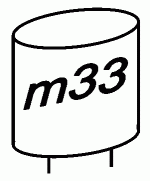
\includegraphics[width=1.1cm]{TC203.png}
}%Frage
{$3,3\mu F$}%A
{$33\mu F$}%B
{$33000\mu F$}%C
{$330\mu F$}%D
{D}%Lösung

\mucho{10}{TC205}
{Welche Kapazität hat der abgebildete Kondensator?\\
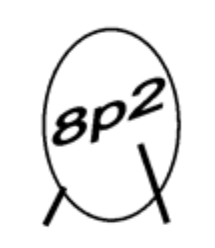
\includegraphics[width=1.1cm]{TC205.png}
}%Frage
{$820pF$}%A
{$8,2pF$}%B
{$82pF$}%C
{$0,82pF$}%D
{B}%Lösung

%%%%%%%%%%%%%%%%%%%%%%%%%%%%%%%%%%%%%%%%%%%%%%%%%%%%%%%%%%%%%%%%%%%%%%%%
%% Praxis

\clearpage

\section{Kapazität}

Der Kondenstator steht als Bauteil stelltvertretend für das Phänomen der
elektischen Kapazität. Im Folgenden soll dieser weiter praktisch untersucht
werden.

\paragraph{Vorbereitungsaufgabe}

\emph{-- fakultativ --} Baut aus irgendetwas einen Kondensator und bringt ihn mit.
Vielleicht findet ihr auch noch einen interessanten Kondensator in eurer
Bastelkiste?

\loesung{Besondere Vorbereitungen: Einen großen DrehKo mitbringen zur
Anschauung.}

\paragraph{Material}

% TODO ergänzen
\begin{itemize}
  \item[1x] ModulBus VCap4 (Datenblatt Anlage \ref{att:vcap})
  \item[1x] LC-Meter (Manual Anlage \ref{att:ae20204})
  \item \dots
\end{itemize}

\paragraph{Hinweise}

%FIXME Bedienungsanleitung in die Anlage
Sorgfältig mit den Messgeräten umgehen. Vorher Bedienungsanleitung lesen,
warmlaufen lassen und kalibrieren!

\paragraph{Aufgaben}

% TODO Aufgaben verbessern!
\begin{enumerate}
    \item Betrachtung des Drehkondensators ModulBus VCap4.
    \begin{enumerate}
      \item Was bedeutet VCap?\\
        \loesung{Variable Capacity}
      \item Wie funktioniert der vorliegende DrehKo?\\
        \loesung{Kapazitätsänderung durch Flächenänderung}
      \item Was machen die Trimmer?\\
        \loesung{}
      \item Welche maximale Kapazität bekommt man aus dem Bauteil?\\
        $C_{max} = \dots$ \loesung{}
      \item Welche minimale Kapazität (einstellbar) bekommt man aus dem
        Bauteil?\\
        $C_{min} = \dots$ \loesung{}
    \end{enumerate}
  \item Was gibt es noch so an Kondensatoren? $\rightarrow$ C bauen, berechnen, messen
  %FIXME Funktioniert die Aufgabe? Wechselstromwiderstand relevant für Klasse E?
  \item Wechselstromwiderstand: NF-AC mit Smartphone erzeugen und Durchgänge
    Kondensator + Lämpchen/Lautsprecher testen
\end{enumerate}
